\documentclass{oblivoir}
\usepackage{amsmath,amssymb,amsthm,kotex,mdframed,paralist,kswrapfig}

\newcounter{num}
\newcommand{\prob}[1]
{\newpage\bigskip\noindent\refstepcounter{num}\textbf{문제 \arabic{num})#1}\par}

\newcommand{\ans}{
{\par\medskip\begin{mdframed}
\textbf{풀이 : }
\vspace{0.6\textheight}
\end{mdframed}\par
\raggedleft\textbf{답 : (\qquad\qquad\qquad\qquad\qquad\qquad)}
\par}\bigskip\bigskip}

\newcommand\ov[2]{\ensuremath{\overline{#1#2}}}

%%%
\begin{document}
\setcounter{page}{0}
\title{기훈 02 - 벡터 문제들.ilpoomsuhak}
\author{}
\date{\today}
\maketitle
%\tableofcontents

\prob{\#285}
\kswrapfig[Pos=r]{01}{
오른쪽 그림의 삼각형 \(ABC\)에서 \(\overline{AB}=3\), \(\overline{BC}=4\)이고 \(\overline{AC}=2:1\)로 내분하는 점을 \(D\)라고 하자.
\(\overline{AB}\)와 \(\overline{BC}\) 위에 \(\overline{BE}:\overline{BF}\)를 \(3:2\)를 만족시키는 두 점 \(E\), \(F\)를 각각 잡고 \(\overline{BD}\)와 \(\overline{EF}\)의 교점을 \(G\)라 할 때, \(\frac{\overline{EG}}{\overline{GF}}\)의 값은?
}
\ans

\prob{}
\kswrapfig[Pos=r]{02}{
오른쪽 그림의 삼각형 \(ABC\)에서 \(\overline{AB}=3\), \(\overline{BC}=5\)이고 \(\overline{AC}=2:1\)로 내분하는 점을 \(D\)라고 하자.
\(\overline{AB}\)와 \(\overline{BC}\) 위에 \(\overline{BE}:\overline{BF}\)를 \(4:3\)를 만족시키는 두 점 \(E\), \(F\)를 각각 잡고 \(\overline{BD}\)와 \(\overline{EF}\)의 교점을 \(G\)라 할 때, \(\frac{\overline{EG}}{\overline{GF}}\)의 값은?
}
\ans

\prob{}
\kswrapfig[Pos=r]{03}{
오른쪽 그림의 삼각형 \(ABC\)에서 \(\overline{AB}=5\), \(\overline{BC}=7\)이고 \(\overline{AC}=3:2\)로 내분하는 점을 \(D\)라고 하자.
\(\overline{BC}\) 위에 \(\overline{BF}=4\)가 되도록 점 \(F\)를 잡고 \(\overline{BD}\)와 \(\overline{EF}\)의 교점을 \(G\)라 할 때,
%\(\overline{AB}\)와 \(\overline{BC}\) 위에 \(\overline{BE}:\overline{BF}\)를 \(3:2\)를 만족시키는 두 점 \(E\), \(F\)를 각각 잡고 \(\overline{BD}\)와 \(\overline{EF}\)의 교점을 \(G\)라 할 때, 
\(\frac{\overline{AG}}{\overline{GF}}\)의 값은?
}
\ans

\prob{}
\kswrapfig[Pos=r]{04}{
오른쪽 그림의 삼각형 \(ABC\)에서 \(\ov BC\)를 \(3:5\)로 내분하는 점을 \(D\), \(\ov AB\)를 \(2:3\)으로 내분하는 점을 \(E\)라고 하자.
\(F\)는 \(\ov AD\)와 \(\ov CE\)의 교점일 때, \(\ov EF:\ov CF\)를 구하시오.
}
\ans

\prob{}
다음 그림에서 \(\ov AD=\ov DE=\ov EC\), \(\ov BF:\ov CF=1:2\)이다. \(a=\frac{\ov BG}{\ov GE}\), \(b=\frac{\ov DG}{\ov GF}\)일 때, \(ab\)의 값을 구하시오.
\begin{figure}[h]
\center
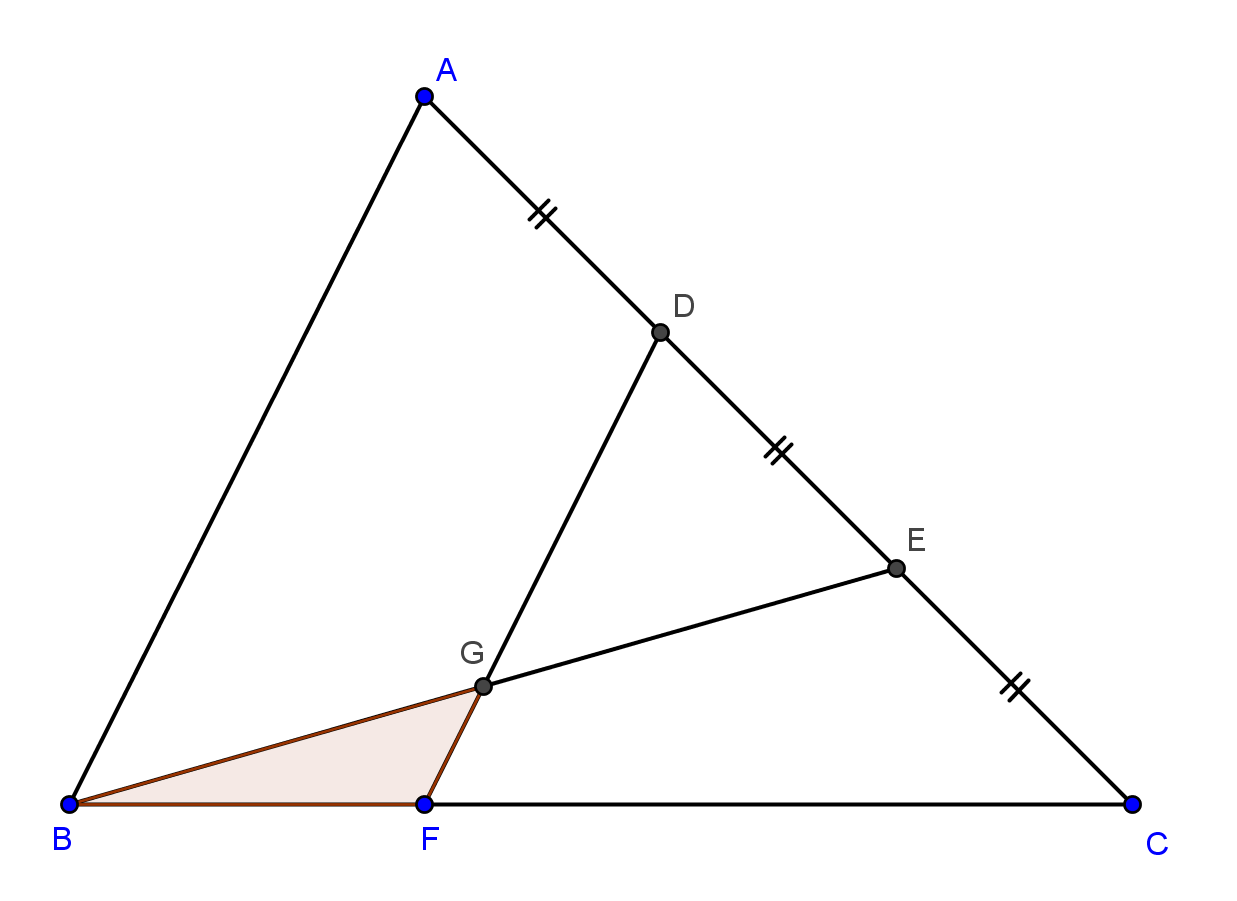
\includegraphics[width=0.5\textwidth]{05}
\end{figure}

{\par\medskip\begin{mdframed}\textbf{풀이 : }\vspace{0.4\textheight}\end{mdframed}\par
\raggedleft\par}\textbf{답 : (\qquad\qquad\qquad\qquad\qquad\qquad)}\par

%
\prob{\#287}
\kswrapfig[Pos=r]{06}{
오른쪽 그림과 같이 삼각형 \(OAB\)에서 \(\overline{OA}\)를 \(2:1\)로 내분하는 점을 \(C\), \(\overline{OB}\)를 \(1:3\)으로 내분하는 점을 \(D\), \(\overline{AD}\)와 \(\overline{BC}\)의 교점을 \(P\)라 할 때, \(\overrightarrow{OP}=a\overrightarrow{OA}+b\overrightarrow{OB}\)이다.
실수 \(a\), \(b\)에 대하여 \(a+b\)의 값은?
}

\ans

%
\prob{}
\kswrapfig[Pos=r]{07}{
오른쪽 그림과 같이 삼각형 \(OAB\)에서 \(\overline{OA}\)를 \(1:2\)로 내분하는 점을 \(C\), \(\overline{OB}\)를 \(1:1\)으로 내분하는 점을 \(D\), \(\overline{AD}\)와 \(\overline{BC}\)의 교점을 \(P\)라 할 때, \(\overrightarrow{OP}=a\overrightarrow{OA}+b\overrightarrow{OB}\)이다.
실수 \(a\), \(b\)에 대하여 \(a+b\)의 값은?
}

\ans

%
\prob{}
\kswrapfig[Pos=r]{08}{
오른쪽 그림과 같이 삼각형 \(OAB\)에서 \(\overline{OA}\)를 \(5:1\)로 내분하는 점을 \(C\), \(\overline{OB}\)를 \(3:1\)으로 내분하는 점을 \(D\), \(\overline{AD}\)와 \(\overline{BC}\)의 교점을 \(P\)라 할 때, \(\overrightarrow{OP}=a\overrightarrow{OA}+b\overrightarrow{OB}\)이다.
실수 \(a\), \(b\)에 대하여 \(a+b\)의 값은?
}

\ans

%
\prob{}
\kswrapfig[Pos=r]{09}{
오른쪽 그림과 같이 삼각형 \(OAB\)에서 \(\overline{OA}\)를 \(4:1\)로 외분하는 점을 \(C\), \(\overline{OB}\)를 \(3:1\)으로 외분하는 점을 \(D\), \(\overline{AD}\)와 \(\overline{BC}\)의 교점을 \(P\)라 할 때, \(\overrightarrow{OP}=a\overrightarrow{OA}+b\overrightarrow{OB}\)이다.
실수 \(a\), \(b\)에 대하여 \(a+b\)의 값은?
}

\ans

%
\prob{}
\kswrapfig[Pos=r]{10}{
오른쪽 그림과 같이 삼각형 \(OAB\)에서 \(\ov OA\)를 \(9:4\)로 외분하는 점을 \(C\), \(\overline{OB}\)를 \(3:1\)으로 내분하는 점을 \(D\), \(\overline{AD}\)의 연장선과 \(\overline{BC}\)의 연장선의 교점을 \(P\)라 할 때, \(\overrightarrow{OP}=a\overrightarrow{OA}+b\overrightarrow{OB}\)이다.
실수 \(a\), \(b\)에 대하여 \(a+b\)의 값은?
}

\ans

%
\prob{\#288}
\kswrapfig[Pos=r]{11}{
오른쪽 그림과 같이 원에 내접하는 사각형 \(ABCD\)의 대각선 \(AC\)가 원의 중심 \(O\)를 지난다.
\(\ov AB=7\), \(\ov AD=9\)일 때, \(\overrightarrow{AC}\cdot\overrightarrow{BD}\)의 값을 구하여라.
}

\ans

%
\prob{\#288}
\kswrapfig[Pos=r]{12}{
오른쪽 그림과 같이 원에 내접하는 사각형 \(ABCD\)의 대각선 \(AC\)가 원의 중심 \(O\)를 지난다.
\(\ov AB=3\), \(\ov AD=6\)일 때, \(\overrightarrow{AC}\cdot\overrightarrow{BD}\)의 값을 구하여라.
}

\ans

%
\prob{\#289}
\kswrapfig[Pos=r]{13}{
오른쪽 그림의 삼각형 \(ABC\)에서 \ov AB의 중점을 \(D\), \ov AC를 \(2:1\)로 내분하는 점을 \(E\), \ov DE 의 중점을 \(F\), \ov AF의 연장선이 \ov BC와 만나는 점을 \(G\)라고 하자.
\ov AG의 길이가 \(24\)일 때, \(\ov AF\)의 길이를 구하여라.
}

\ans

%
\prob{}
\kswrapfig[Pos=r]{14}{
오른쪽 그림의 삼각형 \(ABC\)에서 \ov AB를 \(3:1\)로 내분하는 점을 \(D\), \ov AC의 중점을 \(E\), \ov DE 의 중점을 \(F\), \ov AF의 연장선이 \ov BC와 만나는 점을 \(G\)라고 하자.
\ov AG의 길이가 \(24\)일 때, \(\ov AF\)의 길이를 구하여라.
}

\ans

%
\prob{}
\kswrapfig[Pos=r]{15}{
오른쪽 그림의 삼각형 \(ABC\)에서 \ov AB를 \(1:2\)로 내분하는 점을 \(D\), \ov AC를 \(7:2\)로 외분하는 점을 \(E\), \ov DE 의 중점을 \(F\), \ov AF의 연장선이 \ov BC와 만나는 점을 \(G\)라고 하자.
\ov AG의 길이가 \(24\)일 때, \(\ov AF\)의 길이를 구하여라.
}

\ans

%
\prob{}
\kswrapfig[Pos=r]{16}{
오른쪽 그림의 평행사변형 \(ABCD\)에서 \ov AB를 \(5:3\)으로 내분하는 점을 \(E\), \ov AD를 \(1:2\)로 내분하는 점을 \(F\), \ov EF의 중점을 \(G\), \ov AG의 연장선이 \ov BC와 만나는 점을 \(H\)라고 하자.
\ov AH의 길이가 \(24\)일 때, \(\ov AG\)의 길이를 구하여라.
}

\ans

%
\prob{\#291}
\kswrapfig[Pos=r]{17}{
오른쪽 그림의 색칠한 부분의 넓이를 구하시오
}

\ans

%
\prob{}
\kswrapfig[Pos=r]{18}{
오른쪽 그림의 색칠한 부분의 넓이를 구하시오
}

\ans

%
\prob{}
\kswrapfig[Pos=r]{19}{
오른쪽 그림의 색칠한 부분의 넓이를 구하시오
}

\ans

%
\prob{}
\kswrapfig[Pos=r]{20}{
\textbf{정적분을 이용하여} 오른쪽 그림의 색칠한 부분의 넓이를 구하시오
}

{\par\medskip\begin{mdframed}
\textbf{풀이 : }

(1) \(Q\)의 좌표를 구하시오.

(2) \(f(x)\)를 구하시오.

(3) \(f(x)\)를 적분하여 색칠한 부분의 넓이를 구하시오.
\vspace{0.5\textheight}
\end{mdframed}\par
\raggedleft\textbf{답 : (\qquad\qquad\qquad\qquad\qquad\qquad)}
\par}\bigskip\bigskip

%
\prob{\#299}
삼각형 \(ABC\)에서 실수 \(k\)에 대하여
\[3\overrightarrow{PA}+\overrightarrow{PB}+4\overrightarrow{PC}=k\overrightarrow{AB}\]
를 만족시키는 점 \(P\)가 존재한다.
삼각형 \(PAB\)의 넓이를 \(S(k)\)라 할 때, \(\frac{S(k)}{S(2k)}\)의 값을 구하여라.

\ans

%
\prob{}
삼각형 \(ABC\)에서 실수 \(k\)에 대하여
\[2\overrightarrow{PA}+5\overrightarrow{PB}+\overrightarrow{PC}=k\overrightarrow{AB}\]
를 만족시키는 점 \(P\)가 존재한다.
삼각형 \(ABC\)의 넓이가 \(24\)일 때, 삼각형\(PAB\)의 넓이를 구하여라.

\ans



\end{document}